\documentclass[border=3pt,tikz]{standalone}
\usepackage{amsmath}
\usetikzlibrary {arrows.meta}
\usetikzlibrary {calc}
\begin{document}
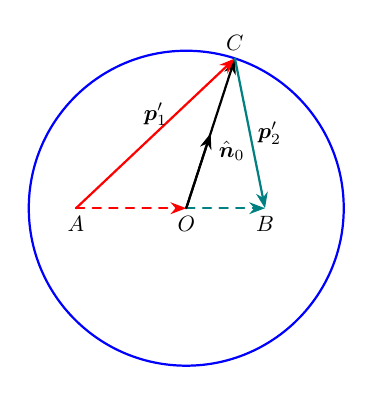
\begin{tikzpicture}[line cap=round, scale = 2]

    \coordinate (A) at (-0.7, 0);
    \coordinate (B) at (0.5, 0);
    \coordinate (C) at (0.309, 0.951);
    
    \draw[fill=none, blue, thick](0,0) circle (1);
    \draw[thick,  -{Stealth[length=2mm]}] (0, 0) node [below, scale=0.8] {$O$} -- (C) node [above, scale=0.8] {$C$};
    \draw[thick, red,  -{Stealth[length=2mm]}] (A) node [below, black, scale=0.8] {$A$} -- (C);
    \draw[thick, teal,  -{Stealth[length=2mm]}] (C) -- (B) node [below, black, scale=0.8] {$B$} ;
    \draw[thick, red, dashed,-{Stealth[length=2mm]}] (A) -- (0, 0);
    \draw[thick, teal, dashed,-{Stealth[length=2mm]}] (0, 0) -- (B);
    
    \draw[thick,  -{Stealth[length=2mm]}] (0, 0)  -- ($0.5*(C)$) node[below right, scale=0.8] {$\hat{\boldsymbol{n}}_0$};
    \node[above,scale=0.8] at ($0.5*(A) + 0.5*(C)$ ){$\boldsymbol{p}'_1$};
    \node[ right,scale=0.8] at ($0.5*(B) + 0.5*(C)$ ){$\boldsymbol{p}'_2$};
    %\node [below, scale=0.8] at ($0.5*(A)$) {$\boldsymbol{p}_A$};
    %\node [below, scale=0.8] at ($0.5*(B)$) {$\boldsymbol{p}_B$};
    
    \end{tikzpicture}
\end{document}